\begin{figure}[h]
    \centering
    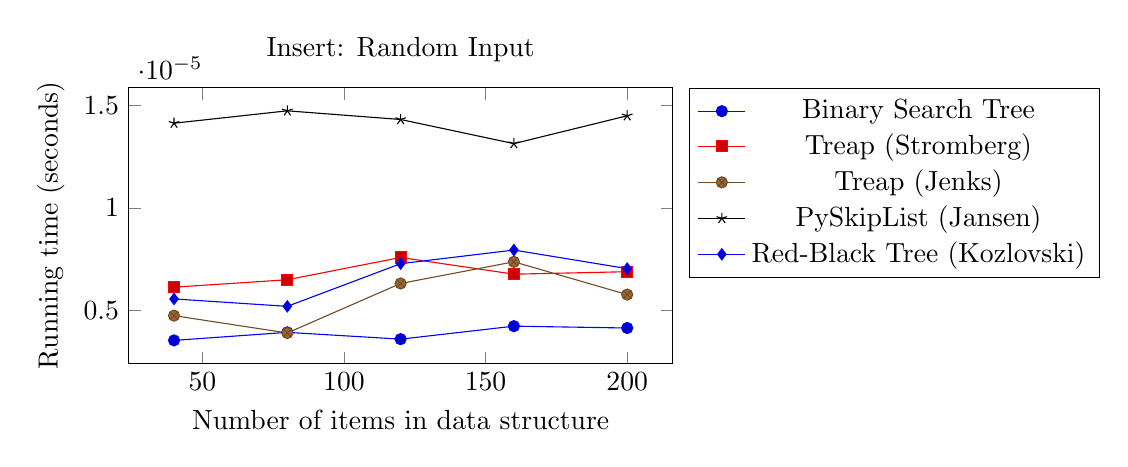
\begin{tikzpicture}
        \begin{axis}[
            xlabel={Number of items in data structure},
            ylabel={Running time (seconds)},
            title={Insert: Random Input},
            width=0.7\textwidth,
            height=2in,
            legend pos=outer north east
        ]
		\addplot coordinates {
			(40, 3.5538689736699937e-06)
			(80, 3.945396911446408e-06)
			(120, 3.6141040410192505e-06)
			(160, 4.2465722481996315e-06)
			(200, 4.1562196471736645e-06)
		};
		\addplot coordinates {
			(40, 6.143976869733836e-06)
			(80, 6.505387273836316e-06)
			(120, 7.589618486142369e-06)
			(160, 6.776445076911442e-06)
			(200, 6.896915211612731e-06)
		};
		\addplot coordinates {
			(40, 4.758570320675948e-06)
			(80, 3.915279377771086e-06)
			(120, 6.324682071784382e-06)
			(160, 7.3787957504165e-06)
			(200, 5.782566465632744e-06)
		};
		\addplot coordinates {
			(40, 1.4125123293654008e-05)
			(80, 1.472747396715629e-05)
			(120, 1.4305828495703165e-05)
			(160, 1.3131244682372533e-05)
			(200, 1.44865336977551e-05)
		};
		\addplot coordinates {
			(40, 5.571743729905488e-06)
			(80, 5.2103333258043946e-06)
			(120, 7.288443149390533e-06)
			(160, 7.951028890243461e-06)
			(200, 7.047502879989343e-06)
		};
        \legend{Binary Search Tree, Treap (Stromberg), Treap (Jenks), PySkipList (Jansen), Red-Black Tree (Kozlovski)}
        \end{axis}
    \end{tikzpicture}
    \caption{Average of 10 operations, benchmarked every 40, starting at 40.}
\end{figure}